%url = https://www.overleaf.com/7690515vynnjrmjmtvc
%url = https://git.overleaf.com/7690515vynnjrmjmtvc


\documentclass[compress]{beamer}

\usetheme{Hamburg}

\usepackage[T1]{fontenc}
\usepackage[utf8]{inputenc}

\usepackage{lmodern}
\usepackage{svg}

%\usepackage[english]{babel}
\usepackage[ngerman]{babel}

\usepackage{eurosym}
\usepackage{listings}
\usepackage{microtype}
\usepackage{units}
\usepackage{minted}
\usepackage{pgfplots}

\usepackage{lineno}
\usepackage{listings}
\usepackage{color}
\usepackage{caption}
\usepackage{listings}
\usepackage{amsmath}
\usepackage{pxfonts}
\usepackage{pgfplots}
\usepackage{pgfplotstable}
\usepackage{filecontents}

\lstset{
	basicstyle=\ttfamily\footnotesize,
	frame=single,
	numbers=left,
	language=C,
	breaklines=true,
	breakatwhitespace=true,
	postbreak=\hbox{$\hookrightarrow$ },
	showstringspaces=false,
	tabsize=4,
	captionpos=b,
	morekeywords={gboolean,gpointer,gconstpointer,gchar,guchar,gint,guint,gshort,gushort,glong,gulong,gint8,guint8,gint16,guint16,gint32,guint32,gint64,guint64,gfloat,gdouble,gsize,gssize,goffset,gintptr,guintptr,int8_t,uint8_t,int16_t,uint16_t,int32_t,uint32_t,int64_t,uint64_t,size_t,ssize_t,off_t,intptr_t,uintptr_t,mode_t}
}

\AtBeginSection[]
{
\begin{frame}
\frametitle{Gliederung (Agenda)}
\tableofcontents[currentsection]
\end{frame}
}

\title{Partikelsimulation}
\author{Oliver Heidmann \& Benjamin Warnke}
\institute{Arbeitsbereich Wissenschaftliches Rechnen\\Fachbereich Informatik\\Fakultät für Mathematik, Informatik und Naturwissenschaften\\Universität Hamburg}
\date{2017-01-12}

\titlegraphic{
\includegraphics[width=0.75\textwidth]{logo}}

\begin{document}

\begin{frame}
	\titlepage
\end{frame}

\begin{frame}
	\frametitle{Gliederung (Agenda)}
	\tableofcontents
\end{frame}
    
\section{Einleitung}
\subsection{}
\begin{frame}%Benjamin
	\frametitle{Ziele}
	\begin{itemize}
		\item Partikel-Simulation für kurzreichweitige Interaktionen
        \item optimiert \& parallelisiert
        \item erweiterbar
        \item Cpp
        \item Auto-Tuning
        \item periodische Ränder
	\end{itemize}
\end{frame}
\section{Theorie}
\subsection{Allgemein}
\begin{frame}%Oliver
	\frametitle{Lennard-Jones-Potential}
    \begin{align*}
	f_{n,i,j}&=\left(\frac{48\epsilon_{i,j}}{\sigma_{i,j}^2}\right)\left[\left(\frac{\sigma_{i,j}}{r_{n,i,j}}\right)^{14}-\frac{1}{2}\left(\frac{\sigma_{i,j}}{r_{n,i,j}}\right)^8\right]r_{n,i,j}
	\end{align*}
\end{frame}
\begin{frame}%Oliver
	\frametitle{Diagramm}
    \begin{figure}
		\begin{center}
			\begin{tikzpicture}
				\begin{axis}[
    	   	 		xmin = 0.5,
    				xmax = 4,
    				xtick = {1,1.5,...,3.5},
    				ymin = -3.5,
    				ymax = 3.5,
   		 			ytick = {-3,...,3},
    				xlabel = $Distanz$, 
        	        ylabel = $Kraft$]
					\addplot[domain=1:4, samples=1000]{(48/1)*((1/x)^14 - 0.5*(1/x)^8)};
				\end{axis}
			\end{tikzpicture}
	    \end{center}
	\end{figure}
\end{frame}
\begin{frame}%Benjamin
	\frametitle{Verlet-Algorithmus}
	\begin{itemize}
		\item basiert auf dem Leapfrog-Verfahren
		\item eliminiert Ungenauigkeiten durch Integration
		\item verringert Abweichungen in den Resultaten zur Realität 
	\end{itemize}
\end{frame}
\begin{frame}%Benjamin
	\frametitle{Verlet-Algorithmus Formel}
    \begin{align*}
	\vec{x}_{1,i}&=\vec{x}_{0,i}+\vec{v}_{0,i}\Delta t+\frac{1}{2}\vec{a}_{0,i}\Delta t^2\\
	\vec{x}_{n+1,i}&=2\vec{x}_{n,i}-\vec{x}_{n-1,i}+\vec{a}_{n,i}\Delta t^2
\end{align*}
\end{frame}
\begin{frame}%Benjamin
	\frametitle{Resultierende Formel}
    \begin{align*}
    A_{i,j}&=48\epsilon_{i,j}\sigma_{i,j}^{12}\Delta t^2\\
	B_{i,j}&=24\epsilon_{i,j}\sigma_{i,j}^{6}\Delta t^2\\
	\vec{x}_{n+1,i}&=\vec{2x}_{n,i}-\vec{x}_{n-1,i}+\sum_{j\in (p\setminus i)}\frac{A_{i,j}-B_{i,j}r_{n,i,j}^6}{r_{n,i,j}^{14}m_i}\left(\vec{x}_{n,j}-\vec{x}_{n,i}\right)
\end{align*}
\end{frame}
\begin{frame}%Benjamin
	\frametitle{Optimierungs Möglichkeiten}
    \begin{itemize}
	    \item kurzreichweitige Interaktionen\\
        	$+$ Zahlendarstellungsungenauigkeiten\\
        	$\rightarrow$ cutoff-radius\\
        	$\rightarrow$ Eliminierung von Berechnungen (kleiner Fehler)
        \item Parallelisierbar
        \begin{itemize}
	        \item OpenMP
            \item CUDA
            \item MPI
        \end{itemize}
    \end{itemize}
\end{frame}
\subsection{Verlet-Listen}
\begin{frame}%Oliver
	\frametitle{Verlet-Listen}
	\begin{itemize}
		\item Nachbarschafts-Listen
        \item berücksichtigt fast nur relevante Partikel
        \item Neuaufbau der Listen alle x Iterationen
		\item Neuaufbau abhängig von momentaner maximalen Geschwindigkeit
        \item sehr geringe Cache-Kohärenz
	\end{itemize}
\end{frame}
\begin{frame}%Oliver
	\begin{figure}
		\begin{center}
			\includegraphics[width=1.0\textwidth]{VerletListDiagramm.png}
		\end{center}
	\end{figure}
\end{frame}
\begin{frame}[fragile]%Oliver
  \begin{minted}[fontsize=\footnotesize]{c++}
// cur = current    // idx = index    // part = particle
void example_iteration()
{
  build_lists_as_explained();

  //for loops over all parts through their indicies
  for(part_idx = 0; part_idx < part_count; part_idx++)
  {
    //loops over all neighbour idx entries
    for(list_idx = 0; list_idx < neighbour_list_size; list_idx++)
    {
      unsigned long cur_neighbour_idx = neighbour_list[list_idx];
      calulate_new_position(
        part_list[cur_part_idx],
        part_list[cur_neighbour_idx]
      );
    }
 }
    \end{minted}
\end{frame}
\subsection{Linked-Cell}
\begin{frame}%Benjamin
	\frametitle{Linked-Cell}
	\begin{itemize}
		\item räumliche Aufteilung des Raums
        \item direkte Umrechnung Position $\leftrightarrow$ Zelle
        \item interagierende Partikel sind im Speicher nahe beieinander \\
        $\rightarrow$ Vektorisierung begünstigt
        \item Vorteil für MPI-Parallelisierung durch Randzellen
	\end{itemize}
\end{frame}
\begin{frame}%Benjamin
	\frametitle{Partikel im Grid}
    \begin{figure}
		\begin{center}
			\includegraphics[height=0.75\textheight]{GridParticles.png}
		\end{center}
	\end{figure}
\end{frame}
\begin{frame}%Benjamin
	\frametitle{Parallelisierung}
    \begin{figure}
		\begin{center}
			\includegraphics[height=0.75\textheight]{GridParallel.png}
		\end{center}
	\end{figure}
\end{frame}
\subsection{Kombination}
\begin{frame}%Oliver
	\frametitle{Verlet-Listen \& Linked-Cell}
	\begin{itemize}
		\item Randübertretungen sind leichter zu erkennen
        \item Neuaufbau ist günstiger durch Zell-Struktur
	\end{itemize}
\end{frame}
\section{Meilensteine}
\subsection{}
\begin{frame}%Oliver
	\frametitle{Hier stehen wir}
	\begin{itemize}
    	\item Planung
    	\item Parameter zum Programmstart
        \item Laden (csv) \& Generieren der Startdaten
        \item Implementation von Lennard-Jones mit dem Verlet-Algorithmus
        \item Datenausgabe (csv, avi)
		\item erste Simulationsdurchl"aufe
        \item Unit-Tests
	\end{itemize}
\end{frame}
\begin{frame}%Oliver
	\frametitle{TODOS}
	\begin{itemize}
        \item Partikel sollen im Feld bleiben
        \item Kombination von Verlet-Listen \& Linked-Cell
		\item  Auto-Tuning
        \item Datenausgabe (verbreitete Formate \& binär)
        \item prüfen der Energieerhaltung
        \item Parallelisierung
	\end{itemize}
\end{frame}
\section{Klassendiagramm}
\subsection{}
\begin{frame}%Benjamin
	\frametitle{Klassendiagramm}
    \begin{figure}
		\begin{center}
			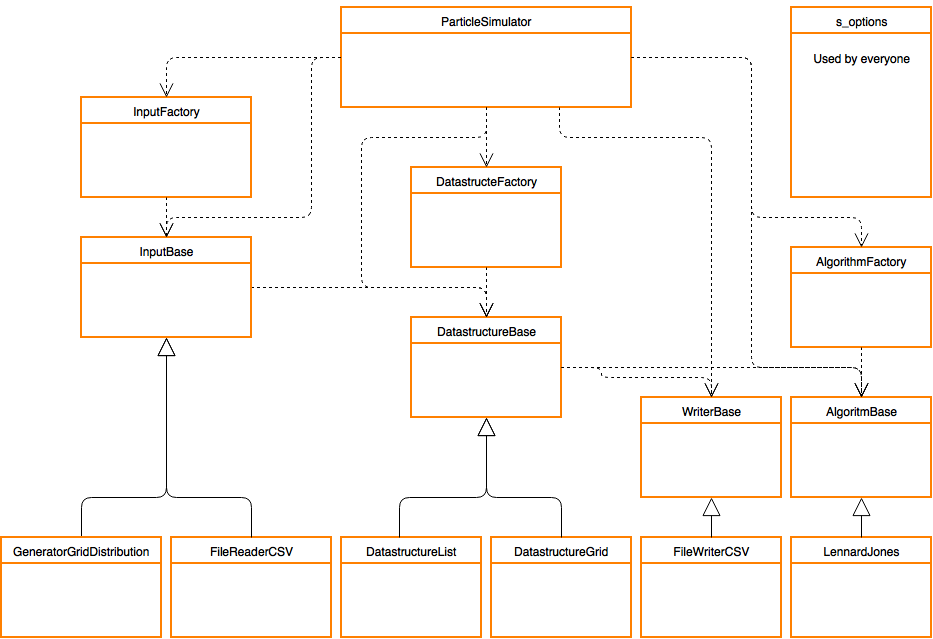
\includegraphics[width=0.9\textwidth]{ClassDiagram.png}
		\end{center}
	\end{figure}
\end{frame}
\section{Output}
\subsection{}
\begin{frame}[fragile]%Oliver
	\frametitle{Output File}
\begin{lstlisting}[caption=data.0.csv]
"ID","PositionX","PositionY","PositionZ"
0, 		1.5,		2.0,		2.0
1,		3.5,		2.0,		2.0
\end{lstlisting}
\end{frame}
\begin{frame}%Benjamin
	\frametitle{Parameter für das Program}
	\begin{itemize}
    	\item algorithm=LENNARD\_JONES
        \item data\_structure=GRID
        \item max\_iterations=7090
        \item write\_fequency=10
        \item cut\_off\_radius=2.5
        \item timestep=0.005
        \item bounds=4/4/4
	\end{itemize}
\end{frame}
\section{Literatur}
\subsection{}
\begin{frame}
	\frametitle{Literatur}
	\begin{itemize}
        \item M-Griebel, S. Knapek, G. Zumbuschm, A. Caglar: Numerische Simulation in der Moleküldynamic. Springer, 2003
		\item D.C Rapaport: The Art of Molecular Dynamics Simulation - 2nd edition, Cambridge University Press, 2004
	\end{itemize}
\end{frame}

\end{document}
